\chapter{Proposed Method}
\label{chapter:proposed-method}

This Chapter describes each of the modules that integrate the method used to
create the trading strategy proposed in this work and how their integration is
performed.

\section{Preprocessing a Financial Market using Retracements}
\label{section:preprocessing-a-financial-market-using-retracements}

Many works that propose methods for financial market forecasting or modelling do
not preprocess the time series that represent a financial market \cite{}. As a
consequent, some of the models that try to simulate these markets have an
additional complexity layer to deal with, similarly to the difficulty that a
neural network would encounter at trying to do facial recognition to
un-processed images. For this reason, a facial recognition algorithm needs to be
fed images that have been rotated, scaled down, and reduced in noise by using
image processing algorithms \cite{}. After doing this preprocessing, it is
easier for a modelling algorithm to create a model of a financial market, as it
does not have to waste time and effort at trying to distinguish between noise
and significant data. 

For financial market preprocessing, an option is to use technical indicators:
mathematical calculations that are applied to time series that represent the
historical prices of a financial market. As an example of a technical
indicator's use, a moving average -- a series of averages of different subsets
of the full data set -- can remove the noise in a market by creating a smooth
line that represents each of the data points in the time series, as can be seen
in Figure~\ref{figure:moving-average-noise}. Other technical indicators can
provide other types of insight about a market, such as the market's volatility,
support and resistance levels, and overbought and oversold levels, among others
\cite{}.

\begin{figure}
\caption{Using a moving average to remove the noise from a financial market time
  series} \centering
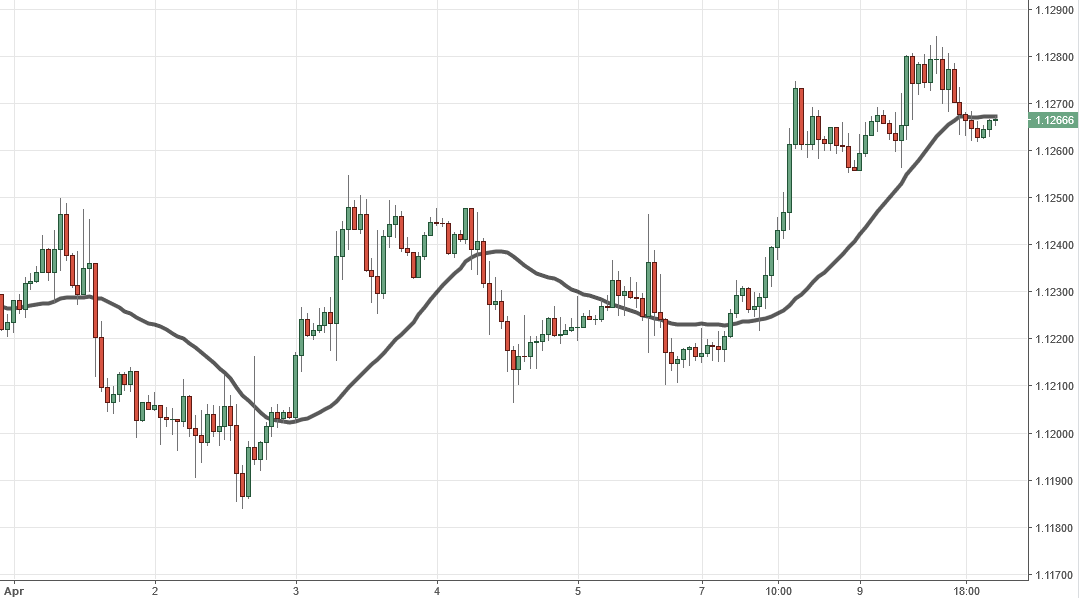
\includegraphics[width=0.7\textwidth]{img/moving-average.png}
\label{figure:moving-average-noise}
\end{figure}

This thesis emphasizes that a financial market's data should always be
preprocessed, and for this reason the proposed method forces this as a
requirement. Although any preprocessing method could be used with the proposed
method, with minimal modifications to the other modules conforming the method, a
preprocessing method that yields multiple insights about the market is
preferred. Additionally, these insights should be numerically represented,
should be continuous and their possible values should encompass an interval. For
example, multiple technical indicators can be used to provide different kinds of
insights. Figure~\ref{figure:multiple-technical-indicators} shows how three
moving averages can be used to represent different perspectives of the market.

\begin{figure}
\caption{Using three moving averages to represent different perspectives of the
  market} \centering
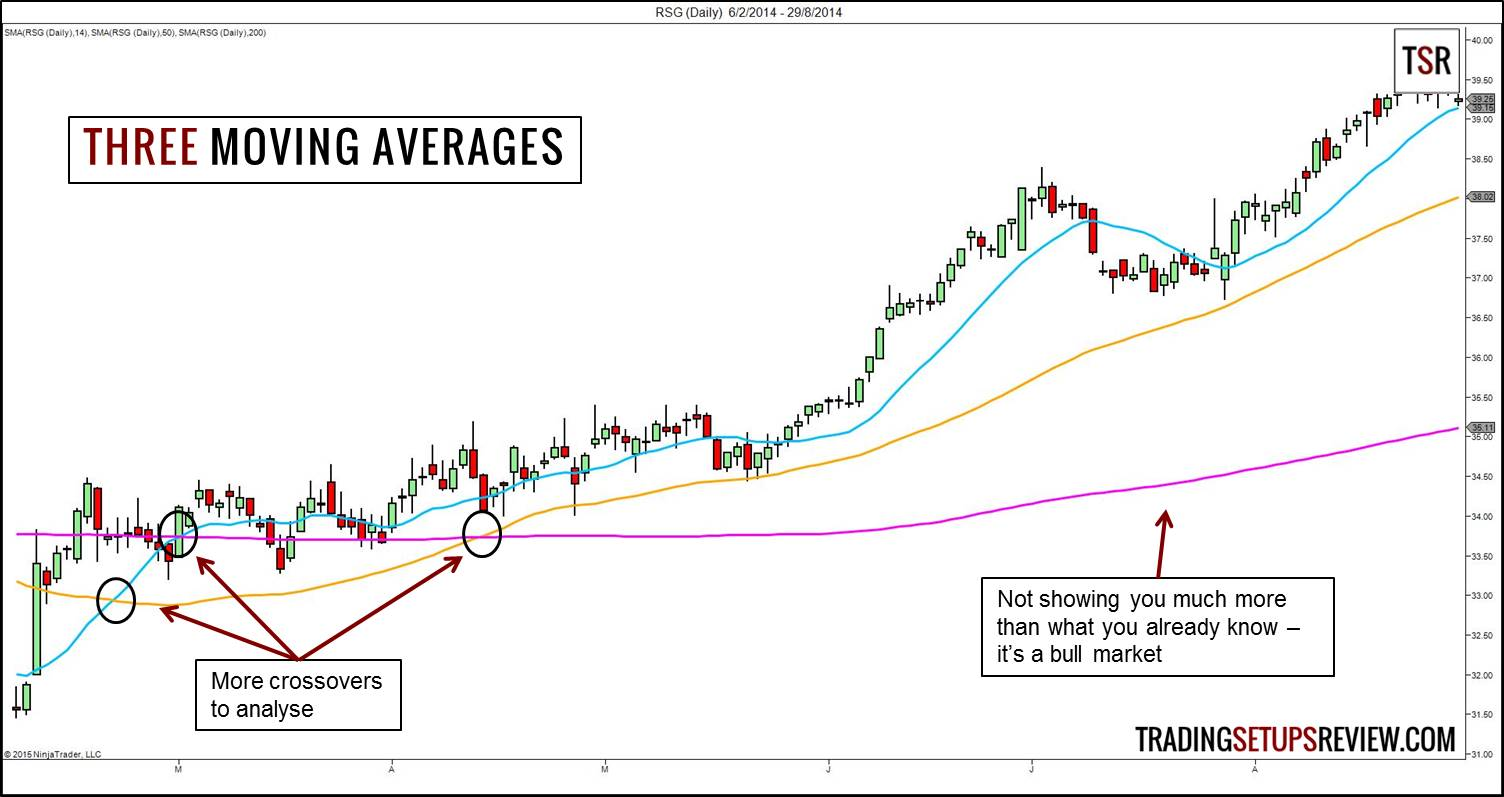
\includegraphics[width=0.7\textwidth]{img/multiple-technical-indicators.jpg}
\label{figure:multiple-technical-indicators}
\end{figure}

The author of this thesis has worked with a variety of technical indicators for
trading a number of financial markets, and has found that support and
resistance-based technical indicators can be used to successfully trade in a
financial market without the use of any other indicators. For this reason, the
proposed method uses a preprocessing algorithm based on this type of technical
indicators. Although it is a subjective reason, it is paramount to note that the
proposed method can easily be adapted to any other preprocessing method; the
preprocessing stage in this work is used mainly in the hopes of facilitating the
agents the interpretation of the market, and thus facilitate the creation of a
model that simulates the market. The backbone idea of this method is to apply a
series of retracements to each of the price differences in a data set. These
price differences are described by \ref{eq:price-differences}.

\begin{equation}
  \label{eq:price-differences}
  \bm{\Delta} = \{ P_1 - P_0, P_2 - P_1, \ldots P_n - P_{n-1} \}
\end{equation}

For example, if the Fibonacci ratios $0.236$, $0.382$ and $0.618$ are used to
generate retracements for the time series $1.35$, $1.36$, $1.34$ and $1.35$ the
values $1.36236$, $1.36382$ and $1.3661801$ are obtained for the first price
difference; $1.3352801$ $1.33236$ and $1.32764$ for the second price difference;
and $1.35236$, $1.35382$ and $1.3561801$ for the last price difference.

Traders normally calculate a single set of retracements for a subset of prices
(see Figure \ref{figure:fibonacci-retracements-in-financial-market}). In
contrast, the process explained in the previous paragraphs calculates multiple
sets of retracements for each of the price differences in a subset of
prices. Figure \ref{figure:retracements-one-price} depicts a plot of the
retracements represented as gray horizontal lines for the previous 200 price
differences from the last price point. In case this is a grayscale printed copy,
the lines that are shorter in width are retracements and the longer ones are
guidelines printed every multiple of $0.0010$.

\begin{figure}
\caption{Retracement lines observed at a singe time point} \centering
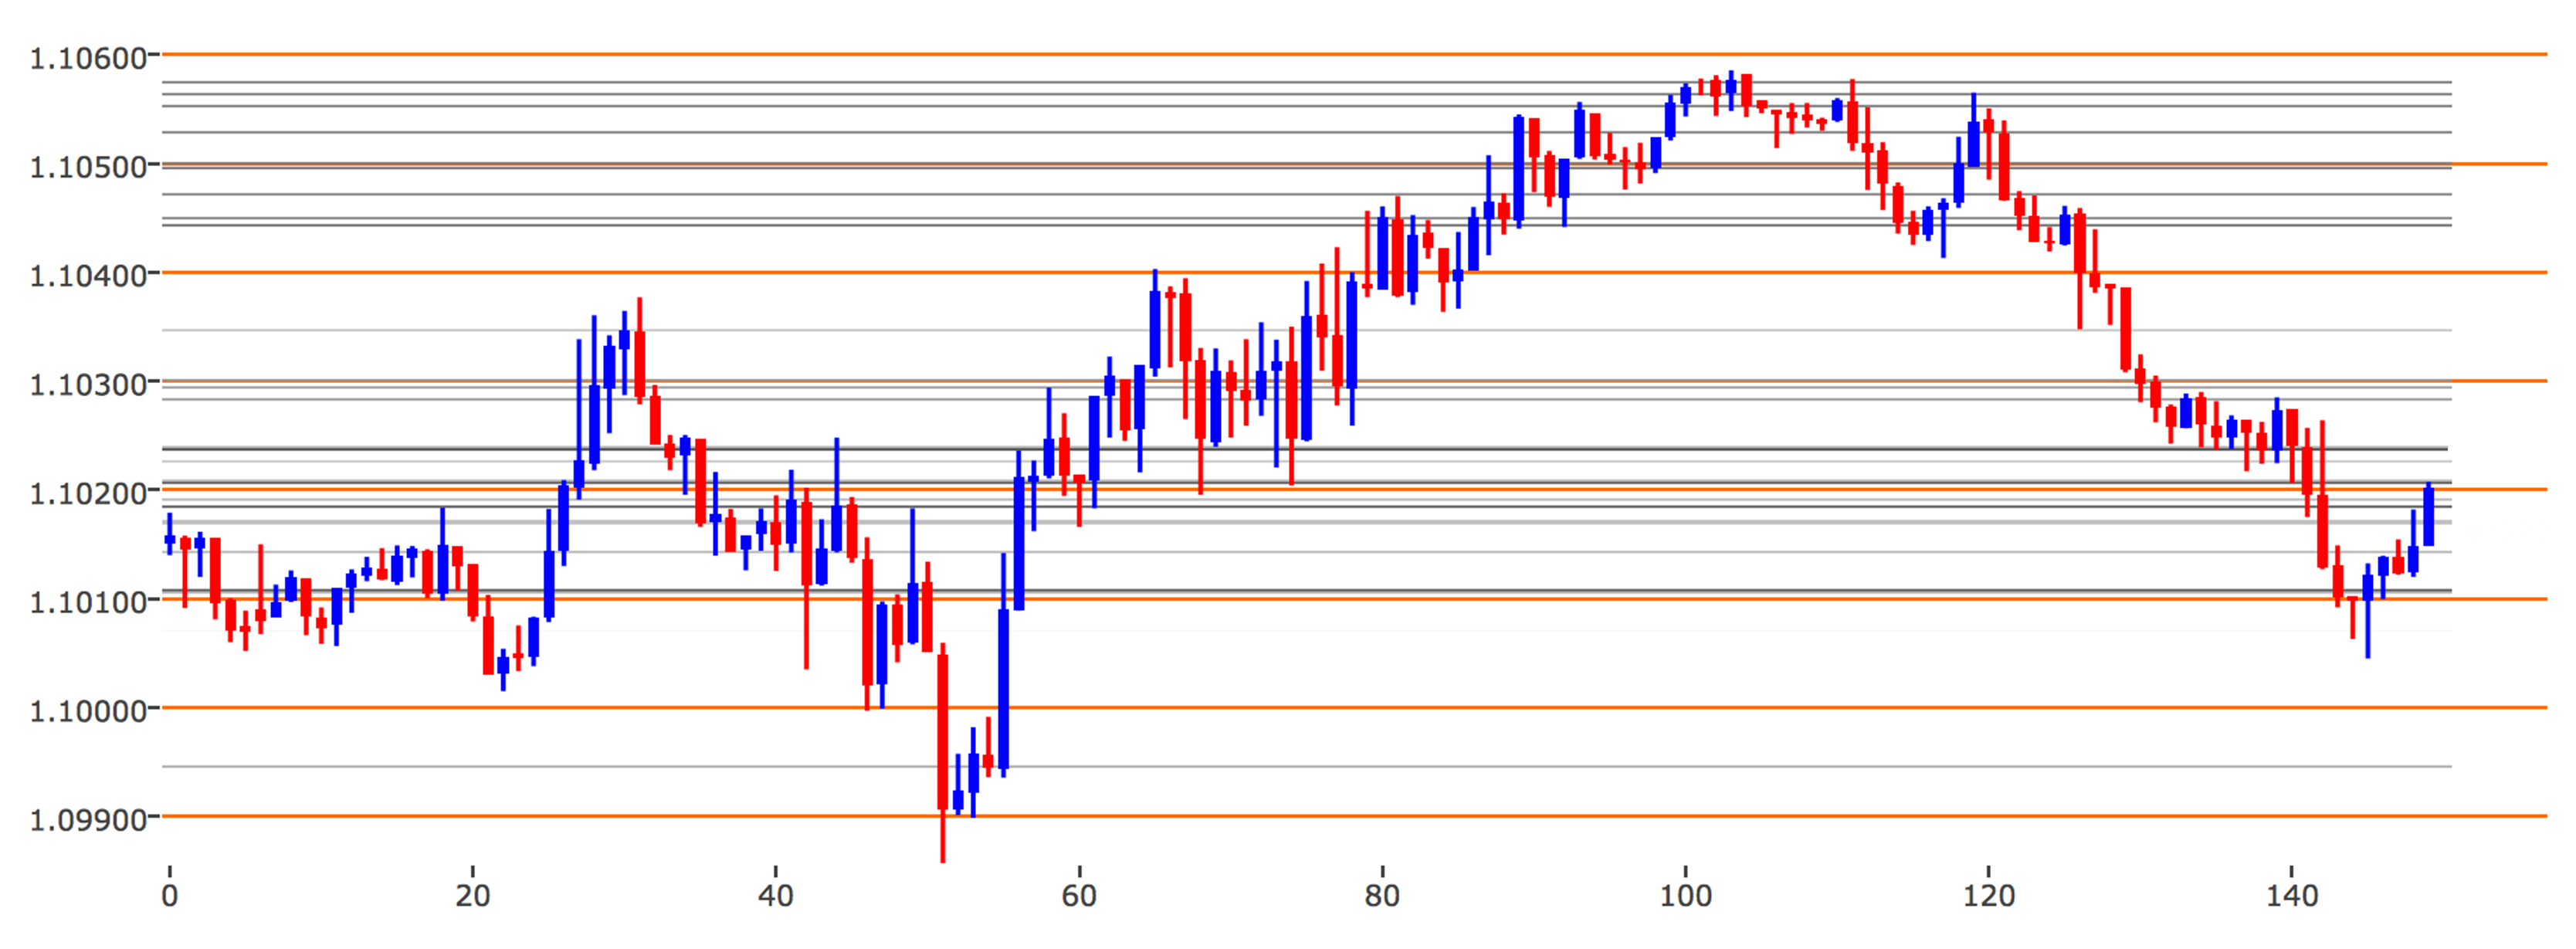
\includegraphics[width=0.7\textwidth]{img/retracements-preprocessing-one-price.png}
\label{figure:retracements-one-price}
\end{figure}

After applying the preprocessing algorithm based on retracements, multiple sets
of retracements are obtained, one for each of the price differences in the
prices subset. Some of these retracements will be duplicates and, for this
reason, a weight is associated to the retracements. If a retracement is found
$n$ times, then the retracement will be associated with a weight of $n$. As canb
e seen in Figure \ref{figure:retracements-one-price}, some retracements are of a
darker color than others -- this color saturation is a graphical representation
of the retracement's weight. Retracements with a greater weight should be trated
as of greater importance, i.e. it should be more common to see a price reversal
or stagnation around such retracement.

As can be noted in Figure \ref{figure:retracements-one-price}, the retracements
plotted are only relevant to a single price point -- the last one. Retracements
at each of the prices in a time series can be plotted if one uses a heatmap
chart, as the one found in Figure
\ref{figure:retracements-all-prices}. Additionally, the latter Figure also
groups all the retracements into 10 unit-areas or, in other words, instead of
having weighted retracement prices now the plot is showing weighted retracement
price intervals. This retracement aggregation is paramount for the proposed
method, as the market data becomes more simplified and easier to read for the
agents: each square in the heatmap represents the influence of the past 200
price points, for a set of 10 different price levels.

\begin{figure}
\caption{Retracement lines observed for every time point} \centering
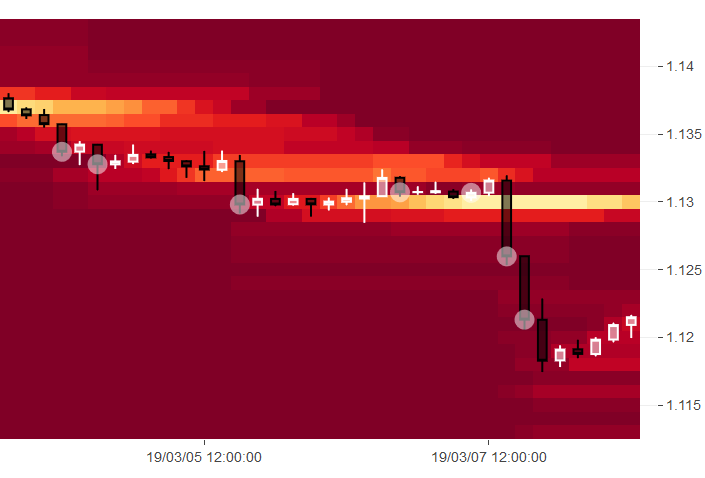
\includegraphics[width=0.7\textwidth]{img/retracements-preprocessing-all-prices.png}
\label{figure:retracements-all-prices}
\end{figure}

\section{Using Agents to Represent Traders in a Financial Market}
\label{section:using-agents-to-represent-traders-in-a-financial-market}

Using an agent-based model to represent a financial market is perhaps one of the
most natural ways to do so. The explanation for this is that any financial
market is, in fact, being constructed by a group of agents: the traders. In the
proposed method, agents follow the process depicted in Figure
\ref{figure:agent-architecture}.

\begin{figure}
\caption{Architecture of an agent} \centering
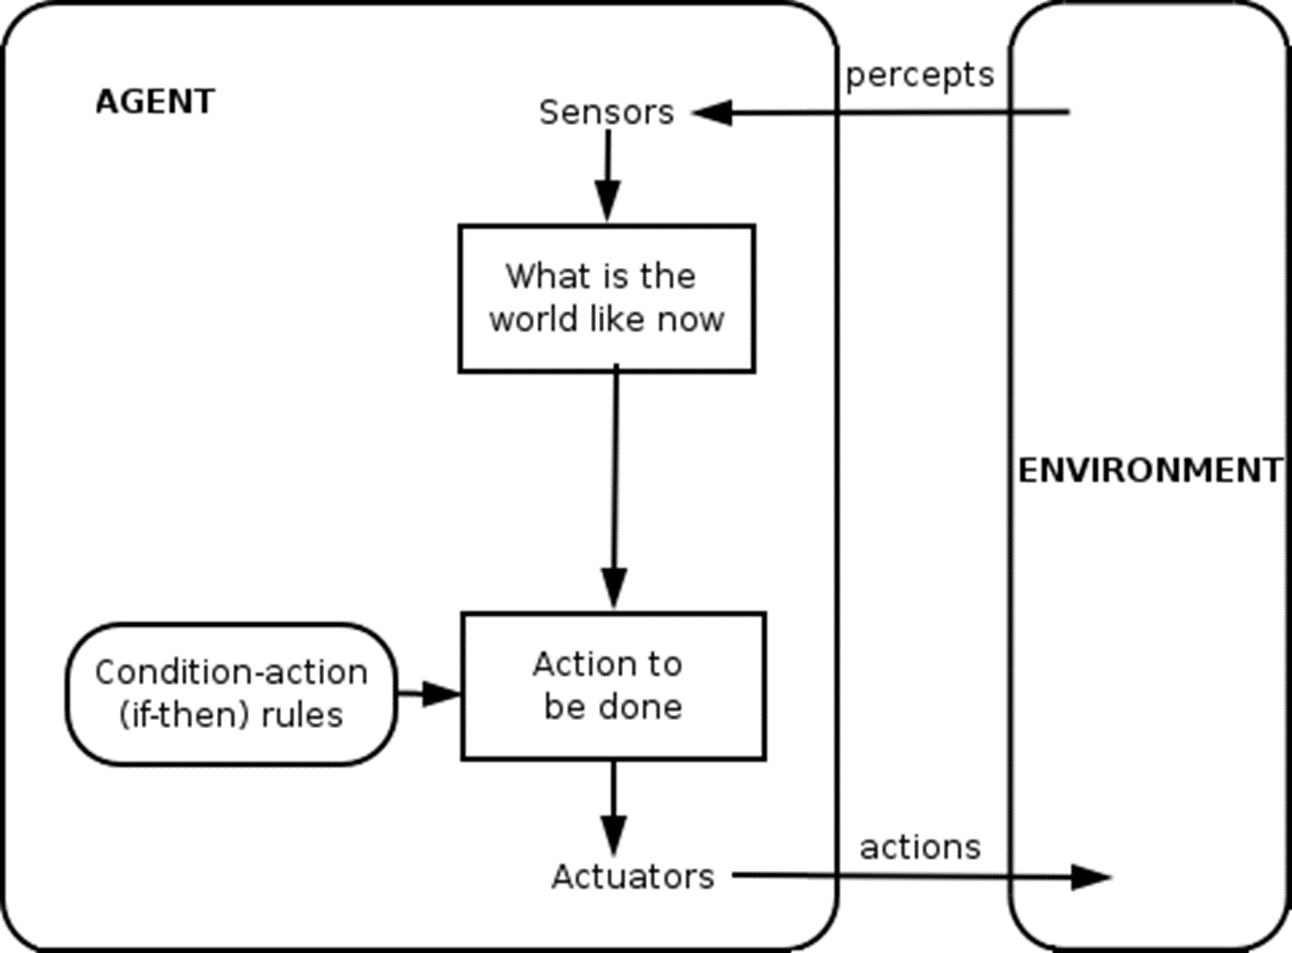
\includegraphics[width=0.7\textwidth]{img/agent-architecture.png}
\label{figure:agent-architecture}
\end{figure}

In this architecture, an agent is constantly sensing its environment, which, in
the case of this thesis, is the raw market prices coming from a broker. The
preprocessing mentioned in Section
\ref{section:preprocessing-a-financial-market-using-retracements} takes place as
part of each agent's sensing process; in other words, each agent has the
capability of preprocessing the market's raw data in their own fashion.

After preprocessing the raw data, each agent uses a set of rules in order to
decide if it should interact with its environment in a certain way. In this
case, this interaction takes the form of trades: the agent decides if it is
necessary to perform a sell or buy transaction for a particular number of units,
or if no action should be performed at all.

The collection of every agent's actions can provide a simulation of the next
market's price. This simulation is achieved by summing each of the agent's
response to the market. In other words, the simulated price for a time $t_0$ can
be obtained by the calculation represented by \ref{equation:sum-of-agents-units}:

\begin{equation}
  \label{equation:sum-of-agents-units}
  p_{t0} = p_t-1 + \sum_{i=1}^{N} U_i
\end{equation}

where $p_{t-1}$ represents the previous price, i.e. the price for time $t_{-1}$, and
$U$ denotes the number of units an agent will trade at time $t_0$. The number of
units can either be positive or negative. This model can successfully represent
how a number of trades in different directions and magnitudes can move the price
of a market.

\section{Using Retracements to Represent the Beliefs of a Trader}
\label{section:using-retracements-to-represent-the-beliefs-of-a-trader}

As mentioned in Section
\ref{section:using-agents-to-represent-traders-in-a-financial-market}, each
trader in the agent-based model can have its own interpretation of the market,
represented by the preprocessing it performs on the market's raw price data. In
order to achieve these market interpretations, the proposed method follows the
ideas proposed by Shoham in \cite{Shoham1993}, where agents have a set of
beliefs that influence how they perceive their environment.

This work proposes that the beliefs of an agent can be represented by the
parameters of their environment preprocessing algorithm. As described in 
Section~\ref{section:preprocessing-a-financial-market-using-retracements}, 
retracements
are used to achieve this preprocessing in the proposed method, which means that
the agents in the agent-based model use as their beliefs a set of ratios that
are used to obtain the retracements in the market. These retracements are then
used to represent prices where the agent believes that a trade could be
initiated. As a consequent, even if two agents have the same trading strategy,
i.e the same rules, they can trade differently depending on how they perceive
the market according to their beliefs.

\section{Representing the Agents' Rules as Intuitionistic Fuzzy Systems}
\label{section:representing-the-agents-rules-as-intuitionistic-fuzzy-systems}

Another concept grabbed from Shoham's work described in \cite{Shoham1993} is
that agents have a set of commitment rules. These commitment rules -- or just
rules, as they will be referred as from now on -- determine what actions, if
any, will an agent perform on their environment.

Some works represent the agents' rules using simple if-then statements
\cite{Niazi2011} \cite{Pellizzari2007}. In contrast, the work in this thesis
uses intuitionistic fuzzy systems to represent the rules. The reason behind this
decision is that fuzzy systems are particularly useful for knowledge
visualization and interpretation. One can examine the membership functions in
the fuzzy rules to have an idea of how the fuzzy system will perform. This can
also be said about simple if/else statements, but fuzzy systems have the
advantage of being able to represent a virtually infinite number of if/else
statements in a simple way (through membership functions) and that they can
easily be optimized using a meta-heuristic algorithm.

In the proposed method, the outputs from the preprocessing algorithm serve as
inputs for the fuzzy system. For example, at certain time point in a market, one
can use the values of different moving averages as the inputs for the fuzzy
system of an agent. The outputs of the preprocessing algorithm are then
associated to a set of membership functions that act as the antecedents of an
inference system which, following the workflow of a common fuzzy system, fire
the membership functions that act as consequents which represents a number of
units that will be traded by the agent at a particular time in the market. It is
noteworthy that in this case Mamdani systems are being proposed to be used as
the agent rules (see Subsection \ref{subsection:fuzzy-systems}). This approach
also provides flexibility, as the system can easily be adapted to any number of
inputs coming from the preprocessing algorithm.

\subsection{Indeterminacy or Hesitancy}
\label{subsection:indeterminacy-or-hesitancy}

The fuzzy systems used to represent the agent rules are of a kind called
intuitionistic fuzzy systems (see Subsection
\ref{subsection:intuitionistic-fuzzy-systems}). This type of fuzzy system
provides an additional abstraction layer to the uncertainty that can be modelled
by traditional fuzzy systems, which is denoted as indeterminacy or hesitancy
\cite{Atanassov1986}. In the case of this work, hesitancy can be seen as doubt
in an agent's perceptions and actions. For example, an agent can be perceiving a
very strong resistance area in the market above the current price, but if the
membership function associated to that input is high, it can mean that the agent
is unsure of what it is perceiving. This perception can be described in words as
``the agent is very unsure of perceiving a high resistance above the current
price''. This previous statement also helps the understanding of the difference
between uncertainty and indeterminacy in an intuitionistic fuzzy system.

As an additional example, one can examine the intuitionistic fuzzy set depicted
in Figure \ref{figure:indeterminacy-in-an-agents-action}. If this fuzzy set
represents the action of an agent (the units to be traded), it can be seen that
the trader is doubtful about trading a moderate number of units. It can also be
seen that this doubt is located at the left of the membership function, which
will cause a trader to be doubtful about trading a below moderate number of
units or, in other words, it will be trading a higher than moderate number of
units. Indeterminacy in this case can model situations such as ``according to
what I'm perceiving, I should be conservative and trade the usual amount of
units. However, taking some additional risk could be worth it, so I will
increase my bet.''

\begin{figure}
\caption{Indeterminacy in an agent's action} \centering
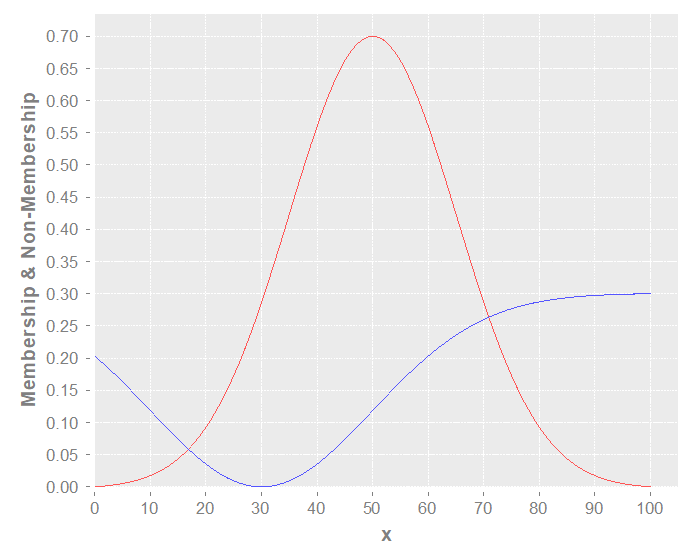
\includegraphics[width=0.7\textwidth]{img/example-of-ifs.png}
\label{figure:indeterminacy-in-an-agents-action}
\end{figure}

Indeterminacy is used in this work to further describe and understand how the
agents in the system are behaving in order to simulate the financial market. As
seen in the results presented in Chapter \ref{chapter:experiments}, a market
report is generated, which summarizes what the agents are perceiving and how
they are responding to their environment. This report also includes the
indeterminacy in these perceptions, which helps the reader understand the role
of doubt in the agents' decisions.

\section{Generation of an Agent-Based Model}
\label{section:generation-of-an-agent-based-model}

Previous Sections describe the architecture and behavior of an isolated
agent. This Section explains how multiple instances of the proposed agent
architecture create an agent-based model of a financial market.

As has been explained, an agent in the proposed method interacts with its
environment by issuing trade orders. These trade orders can be one of two
possible types: buy or sell. If an agent buys units of an asset, the price of
said asset rises. In contrast, if an agent sells units, the price declines. This
conception can be extended to multiple agents trading the same asset: if there
is a majority of units being bought in an asset, the price rises, and it
declines if the majority is selling the asset. The process aforementioned can be
used to create a simulation of a market, where the agents in a multi-agent
system need to be adjusted to create a zero-sum situation that fits the real
market prices. For example, if the price difference between the price at $t_n$
and the price at $t_{n+1}$ is -10 units, the sum of the units traded by all the
agents must be equal to those -10 units.

In the case of simulating a single price, the adjustment of the multi-agent
system becomes trivial, but the complexity of the model grows exponentially as
more prices are added to the simulation. If one price is added, the system needs
to be able to simulate it correctly and all the previous prices, i.e. the
readjustment not only needs to consider the new price, but all the prices as a
whole.

This work proposes that a meta-heuristic is used to find a combination of
parameters that adjusts the multi-agent system in order to perform a
sufficiently good simulation of a real market. This combination of parameters is
composed of the beliefs and the rules of all the agents in the system. One way
to achieve exploitation in the meta-heuristic is to recombine the beliefs and
the rules among each of the agents, however, the exploration capacity of the
algorithm would be limited, as this situation would be similar to performing
crossover on a single chromosome. This becomes clearer after remembering that
each of the agents do not correspond to a solution to the system, but rather
every agent in the system create a solution or a model. As a consequent,
multiple communities of agents need to be created, and the collections of
beliefs and rules of each of the agents in the communities of agents are used in
the recombination process of the meta-heuristic.

The performance of a community of agents can be determined by any function that
can be used in curve-fitting problems, such as the mean-squared error. The
multi-agent to be evaluated is executed to simulate a set of prices that
correspond to a real financial market, and this simulation is then compared to
the real prices. It is not critical for the system to achieve a low
curve-fitting error (for example, a low mean-squared error), as it is desirable
for the system to provide a generalized model of the market. In other words, one
should not seek an overtraining situation, as the system will not be able to
correctly extrapolate its simulation to similar situations.

\section{Using the Agent-Based Model to Generate Insights about a Financial
Market}
\label{section:using-the-agent-based-model-to-generate-insights-about-a-financial-market}

Once an agent-based model of a financial market has been created, this model can
be examined to obtain information about the market. This process is possible
thanks to the agent-based architecture of the model, as the beliefs of the
agents provide an abstraction of what the traders in the real market are
perceiving, and the rules of the agents tell an explanation of the behavior of
the traders. Furthermore, as has been explained in Section
\ref{section:representing-the-agents-rules-as-intuitionistic-fuzzy-systems},
using an intuitionistic fuzzy system to represent the rules of an agent is
helpful in breaking down the different factors that guided an agent to a
decision.

The proposed method can specifically help the user to understand the following
characteristics of the market:

\begin{itemize}
\item \label{item:agents-perception} The number of agents that are perceiving
  the market in some way.
\item \label{item:agents-decisions} The number of agents that are taking certain
  decision according to what they perceived.
\item \label{item:agents-profit} The generated profit per agent in each of the
  training or testing datasets.
\item \label{item:agents-doubt} How doubt or hesitancy is influencing an agent's
  perceptions and decisions
\end{itemize}

\ref{item:agents-perception} is obtained by examining the agents beliefs and/or
the outputs of the preprocessing algorithm associated to these
beliefs. Considering the retracements preprocessing algorithm explained in
Section \ref{section:preprocessing-a-financial-market-using-retracements}, one
can calculate how many agents perceived that a market was experiencing a strong
resistance above the current price, for example. Furthermore, this calculation
can be extended to determine the percentage of the times where these agents
perceived this resistance. In a similar fashion, \ref{item:agents-decisions}
helps the user to describe the trading decisions of the agents: one can
calculate how many agents decided to buy at certain time in the market, and it
can be extended to determine what percentage of the time those agents decided to
take that decision.

\ref{item:agents-profit} is useful to determine the efficacy of an agent, as in
the end one is interested in examining the behavior of the agents that generated
a greater profit than the others, in order to follow its recommendations; or
maybe one can be interested in examining those who performed badly, in order to
avoid taking similar decisions.

Finally, \ref{item:agents-doubt} allows the system to express how sure were the
agents about their perceptions or trade decisions. One can use this doubt
measurement to decide if an economic bubble is approaching, for example, as this
economic phenomenon is caused by factors that are exogenous to the nature of the
financial market \cite{Martin2011}.

\section{Using the Agent-Based Model to create a Trading Strategy}
\label{section:using-the-agent-based-model-to-create-a-trading-strategy}

Using the multi-agent system as a trading strategy is straightforward. After the
system has undergone the optimization process, it should represent a
generalized model of the financial market that was fed to the system as a
training dataset. This training data set encompasses a time period that goes
from $t_{0-n}$ to $t_0$. If the beliefs and rules obtained from the optimization
process still describe the financial market after the aforementioned time
period, then the system is able to forecast the prices comprehending a time
period from $t_0$ to $t_{0+m}$. As a result, a trader that decides to use the
proposed method as a trading strategy should consider the simulated prices as a
guideline on what trading decisions to take.
